\documentclass[10pt,a4paper]{article}

\usepackage{xcolor} % Texto con color
\usepackage{framed} % Enmarcar texto
\usepackage{graphicx} % Imágenes
\usepackage{overpic} % Texto sobre imágenes

\usepackage{pifont} % Símbolos (círculo blanco)

% Márgenes
\usepackage{geometry}
 \geometry{
 a4paper,
 total={175mm,257mm},
 left=15mm,
 top=15mm,
 }

% Fuente
\usepackage{palatino}
%\usepackage{tgpagella}

\definecolor{darkgreen}{rgb}{0,0.7,0} % Verde "normal"
\definecolor{shadecolor}{gray}{0.95} % Para el entorno "shaded" del paquete "framed"

\title{Dragon Ball Super Juego de cartas}
\author{}
\date{}

\begin{document}

\sffamily

\maketitle
%\tableofcontents
%\newpage

\section{\textsf{Introducción}}
  Este es un juego de cartas para dos jugadores. Los jugadores combaten entre sí con barajas de 50 cartas más 1 carta de líder. \newline
  Los jugadores atacan por turnos al líder del oponente. \newline
  Gana el primer jugador que reduzca a cero la vida del oponente.

\section{\textsf{Cómo ganar}}
  \begin{enumerate}
    \item Reducir a 0 la vida del oponente.
    \begin{itemize}
      \color{red} \item Ganas en cuanto no queden cartas en la zona de vida.
    \end{itemize}
    \item Agotar el mazo del oponente.
    \begin{itemize}
      \color{red} \item Cuando se juega con media baraja, los jugadores no pierden cuando se quedan sin cartas. Se baraja la pila de descartes y se vuelve a utilizar como mazo.
    \end{itemize}
  \end{enumerate}

\section{\textsf{Tipos de cartas}}
  \begin{description}
    \item [\textsf{Líder}]
    El líder del equipo, la carta que combate contigo toda la partida.
    Cuando la cosa se complica, la carta despierta, dando la vuelta al dorso más poderoso.
    \begin{center}
%      \begin{overpic}[width=400px,grid,tics=10]{SD1-01ST_both.jpg}
      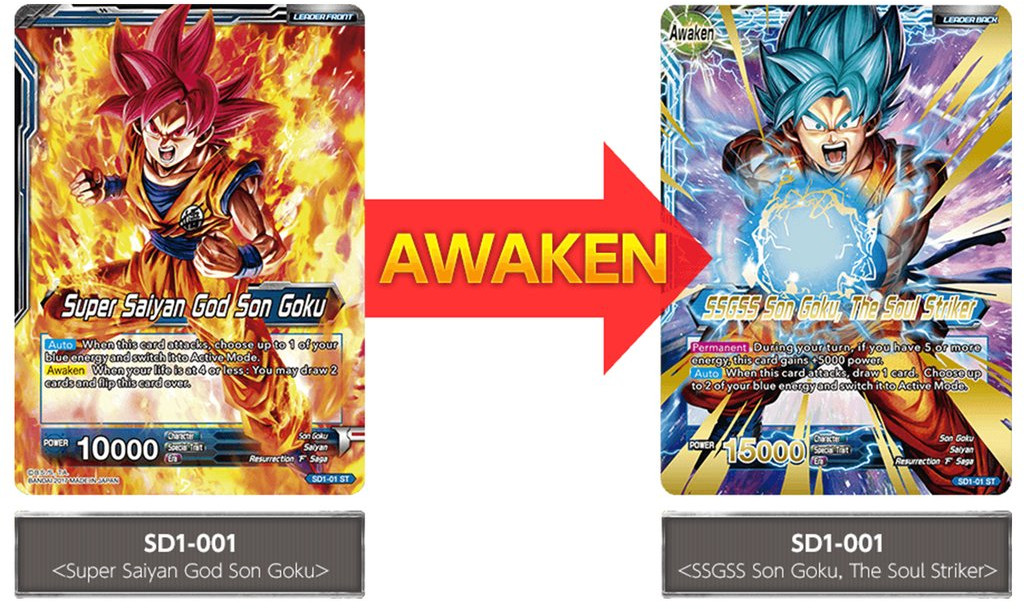
\includegraphics[width=400px]{SD1-01ST_both.jpg}
      \begin{overpic}[width=400px]{SD1-01ST_both.jpg}
        \put (6,29) {\colorbox{red}{\color{white}Nombre de la carta}}
        \put (6,23) {\colorbox{red}{\color{white}Habilidades}}
        \put (7.5,15) {\colorbox{red}{\color{white}Poder}}
        \put (20,17) {\colorbox{red}{\color{white}\tiny{Nombre del personaje}}}
        \put (20,15) {\colorbox{red}{\color{white}\tiny{Rasgo especial}}}
        \put (20,13) {\colorbox{red}{\color{white}\tiny{Era}}}
        \put (22,11) {\colorbox{red}{\color{white}\tiny{Nº carta/Rareza/Color}}}
        \put (63,55.5) {\colorbox{red}{\color{white}\scriptsize{Despertar}}}
      \end{overpic}
    \end{center}

    \item [\textsf{Carta de combate}]
    Estas cartas combaten junto al líder.
    Combaten en la zona de combate y en la zona de combo.
    \begin{center}
      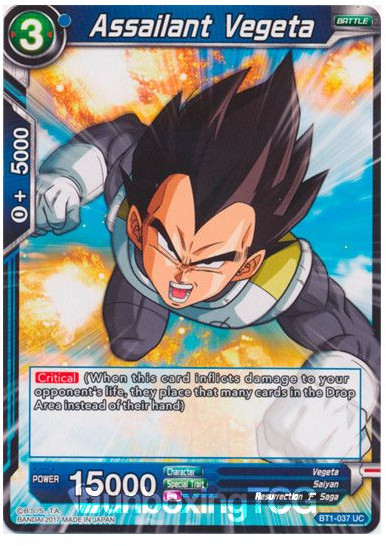
\includegraphics[width=140px]{BT1-037UC.jpg}
      \begin{overpic}[width=140px]{BT1-037UC.jpg}
        \put (0,93) {\colorbox{cyan}{\color{white}\scriptsize{Coste}}}
        \put (12,94) {\colorbox{cyan}{\color{white}Nombre de la carta}}
        \put (60,94) {\colorbox{cyan}{\color{white}\scriptsize{Tipo}}}
        \put (6,71) {\colorbox{cyan}{\color{white}\scriptsize{Poder de combo}}}
        \put (6,59) {\colorbox{cyan}{\color{white}\scriptsize{Coste de combo}}}
        \put (7,26) {\colorbox{cyan}{\color{white}Habilidades}}
        \put (12.5,10) {\colorbox{cyan}{\color{white}Poder}}
        \put (38,15) {\colorbox{cyan}{\color{white}\tiny{Nombre del personaje}}}
        \put (38,11) {\colorbox{cyan}{\color{white}\tiny{Rasgo especial}}}
        \put (38,7) {\colorbox{cyan}{\color{white}\tiny{Era}}}
        \put (41,2) {\colorbox{cyan}{\color{white}\tiny{Nº carta/Rareza/Color}}}
      \end{overpic}
    \end{center}

    \item [\textsf{Carta extra}]
    Estas cartas tienen habilidades que se activan directamente desde la mano.
    Se colocan en la pila de descartes después de usarlas.
    \begin{center}
      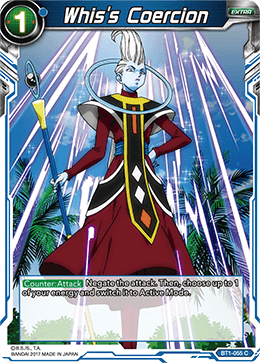
\includegraphics[width=140px]{BT1-055.png}
      \begin{overpic}[width=140px]{BT1-055.png}
        \put (0,93) {\colorbox{cyan}{\color{white}\scriptsize{Coste}}}
        \put (12,94) {\colorbox{cyan}{\color{white}Nombre de la carta}}
        \put (60,94) {\colorbox{cyan}{\color{white}\scriptsize{Tipo}}}
        \put (7,17) {\colorbox{cyan}{\color{white}Habilidades}}
        \put (41,3) {\colorbox{cyan}{\color{white}\tiny{Nº carta/Rareza/Color}}}
      \end{overpic}
    \end{center}
  \end{description}

  \begin{shaded}
    \textbf{Energía (coste)}
    \begin{center}
      \begin{overpic}[width=40px]{energy.jpg}
        \put (100,70) {\colorbox{cyan}{\color{white}\scriptsize{Coste de color}}}
        \put (85,35) {\colorbox{cyan}{\color{white}Coste total}}
      \end{overpic}
    \end{center}
    \textcolor{red}{El número en el centro indica el coste total.} \newline
    La energía usada para pagar el coste debe incluir al menos tantas cartas de color como esferas de color se indiquen en la carta.
  \end{shaded}

\section{\textsf{Desarrollo del juego}}
  \begin{enumerate}
    \item \textbf{Fase de carga}
    \begin{itemize}
      \item Robar una carta
      \item Cargar energía
    \end{itemize}

    \item \textbf{Fase principal}
    \begin{itemize}
      \item Jugar cartas de luchador de la mano
      \item Usar habilidades
      \item Atacar el líder del oponente e infligirle daño
    \end{itemize}

    \item \textbf{Fase final}
    \begin{itemize}
      \item El turno pasa al oponente.
    \end{itemize}
  \end{enumerate}

\section{\textsf{Imprescindible}}
  \begin{enumerate}
    \item Una carta de líder
    \item Baraja de 50 cartas (25 si se juega con media baraja)
  \end{enumerate}

  \begin{shaded}
    \textbf{Reglas de construcción de mazos}
    \begin{itemize}
      \item Un total de 50 cartas entre cartas de luchador y cartas extra
      \item No se permiten cartas de líder en el mazo
      \item Máximo 4 copias de cada carta en el mazo
    \end{itemize}
  \end{shaded}

\section{\textsf{Preparación}}
  \begin{enumerate}
    \item Colocar al líder boca arriba en la zona de líder en posición activo. Colocar el mazo boca abajo en la zona del mazo.
    \item Decidir al azar qué jugador empieza.
    \item Robar 6 cartas del mazo. Estas cartas componen la mano.
    \item Se puede volver a robar una vez (mulligan)
    \begin{itemize}
      \item Devolver cualquier cantidad de cartas al mazo, barajar y volver a robar tantas cartas como se hayan descartado.
    \end{itemize}
    \item Colocar 8 cartas de la parte superior del mazo boca abajo en la zona de vida.
    \begin{itemize}
      \item No se puede mirar las cartas de la zona de vida durante la partida.
    \end{itemize}
    \item Empezar la partida.
  \end{enumerate}

\begin{shaded}
  \textbf{Desarrollo del juego}
  \begin{enumerate}
    \item \textbf{Fase de carga} \newline
    Se realizan las siguentes acciones por orden:
    \begin{enumerate}
      \item Preparar las cartas agotadas.
      \item Robar una carta del mazo. \newline
            \emph{El jugador inicial no puede robar en el primer turno} \newline
            \emph{No hay límite de cartas en la mano}
      \item Jugar una carta de la mano en la zona de energía en modo activo (preparada). \newline
            \emph{No es obligatorio} \newline
            \emph{No hay límite de cartas en la zona de energía}
    \end{enumerate}

    \item \textbf{Fase principal} \newline
    Se puede realizar las siguientes acciones tantas veces como se desee:
    \begin{itemize}
      \item \textbf{Jugar cartas de luchador de la mano} \newline
      Se puede jugar una carta de luchador en la zona de combate en modo activo (preparada) pagando su coste de energía.
      Se puede pagar el coste de una carta girando (agotando) tantas cartas de de energía como indique la carta.
      Si la energía (coste) incluye esferas de color, el pago debe incluir la misma cantidad (o más) de cartas del mismo color. \newline
      \emph{Ejemplo:} si la energía (coste) es (1 rojo, 2 total) hay que pagar el coste agotando (girando) dos cartas en total: una roja y otra de cualquier color.

      \item \textbf{Activar habilidades} \newline
      Se puede activar habilidades de líder, cartas de luchador o cartas extra con \colorbox{orange}{\color{white}Activate: Main} de la mano.
      Las habilidades \colorbox{red}{\color{white}Evolve}, \colorbox{red}{\color{white}EX-Evolve}, \colorbox{red}{\color{white}Xeno Evolve}, \colorbox{red}{\color{white}Union}, \colorbox{red}{\color{white}Over Realm}, \colorbox{red}{\color{white}Dark Over Realm}, \colorbox{red}{\color{white}Swap}, \colorbox{yellow}{Awaken} o \colorbox{yellow}{Wish} se pueden activar en esta fase.
      Si la habilidad indica un coste, se deben cumplir las condiciones para poder activarla. \newline
      \emph{Ejemplo:} si la energía (coste) es (2 rojo, 4 total) hay que pagar el coste agotando (girando) cuatro cartas en total: dos rojas y otras dos de cualquier color. \newline
      Se puede activar cartas extra agotando (girando) su coste energético. Las cartas extra usadas se descartan.
      Se puede activar cartas extra \colorbox{darkgreen}{\color{white}Field}, que quedan en la zona de combate en modo activo.

      \item \textbf{Despertar al líder} \newline
      Se puede girar el dorso del líder si se cumplen las condiciones indicadas.

      \item \textbf{Combatir} \newline
      Se agota (gira) el líder o una carta de luchador y se elige como objetivo el líder del oponente o una de sus cartas de luchador agotadas (giradas).
      \begin{itemize}
        \item Las cartas pueden atacar desde el momento en el que se juegan.
        \item El jugador inicial no puede atacar en el primer turno.
      \end{itemize}
      Atacar inicia un combate. El oponente puede activar \colorbox{red}{\color{white}Blocker} con cualquiera de sus otras cartas. \newline
      \colorbox{red}{\color{white}Blocker} \emph{Cuando atacan a otra carta, se puede agotar (girar) esta carta para establecerla como objetivo del ataque}

      \item \textbf{Ir a la fase final} \newline
      Terminar la fase principal e ir a la fase final.
    \end{itemize}

    \item \textbf{Fase final} \newline
    El turno pasa al oponente.
  \end{enumerate}
\end{shaded}

\begin{shaded}
  \textbf{Combate} \newline
  Atacar inicia un combate. Un combate consta de los siguientes pasos:

  \begin{enumerate}
    \item \textbf{Ataque} \newline
    Se puede realizar las siguientes acciones tantas veces como se desee:
    \begin{itemize}
      \item \textbf{Combo} \newline
      Colocar cartas de luchador de tu mano o de la zona de combate en la zona de combo (ver detalles)
      \item \textbf{Activar habilidades} \newline
      Se puede activar las habilidades \colorbox{orange}{\color{white}Activate: Battle} \newline
      También se puede despertar al líder \colorbox{yellow}{Awaken} o pedir un deseo \colorbox{yellow}{Wish}.
      \item \textbf{Pasar al paso de defensa}
    \end{itemize}
    Tras terminar el paso de ataque, se pasa al paso de defensa.

    \item \textbf{Defensa} \newline
    El oponente puede realizar las siguientes acciones tantas veces como desee:
    \begin{itemize}
      \item \textbf{Combo} \newline
      Colocar cartas de luchador de la mano o de la zona de combate en la zona de combo (ver detalles)
      \item \textbf{Activar habilidades} \newline
      Se puede activar las habilidades \colorbox{orange}{\color{white}Activate: Battle} \newline
      También se puede despertar al líder \colorbox{yellow}{Awaken} o pedir un deseo \colorbox{yellow}{Wish}.
      \item \textbf{Pasar al paso de daño}
    \end{itemize}
    Tras terminar el paso de defensa, se pasa al paso de daño.

    \item \textbf{Daño} \newline
    Se compara el poder de las cartas en este paso. \newline
    Comparar el poder total de la carta atacante y sus cartas de combo con el poder de la carta defensora y sus cartas de combo.
    El bando con más poder gana el combate (en caso de empate, gana la parte atacante) \newline
    Si gana la parte atacante, se hace lo siguiente:
    \begin{itemize}
      \item Si se ha derrotado al líder del oponente, se inflige un punto de daño al oponente. \newline
            \emph{Por cada punto de daño, el oponente roba una carta de su pila de vida a su mano}
      \item Si se ha derrotado un luchador, se noquea esa carta.
            Las cartas noqueadas se descartan en la pila de descartes.
    \end{itemize}

    Se descartan todas las cartas de la zona de combo (de ambos bandos).
  \end{enumerate}

  Con el paso de Daño se finaliza el combate.
\end{shaded}

\begin{shaded}
  \textbf{Combo} \newline
  Se pueden jugar cartas de combate activas de la zona de combate en la zona de combo (esto no se considera jugar cartas de luchador). \newline
  Se suma el poder de las cartas de la zona de combo al poder de las cartas de luchador durante el paso de daño.
  \begin{itemize}
    \item Las cartas de luchador en la mano o en la zona de combate (deben estar activas/preparadas) se pueden jugar en la zona de combo pagando (girando) su coste de energía.
    \item No hay límite al número de cartas que se pueden jugar en la zona de combo.
    \item Se resuelven los combos una carta tras otra.
  \end{itemize}
\end{shaded}

\begin{shaded}
  \textbf{Preguntas frecuentes} \newline

  P1. ¿Qué pasa si se activan a la vez dos habilidades automáticas? \newline
  \emph{R1. Se activan en el orden que se desee.} \newline

  P2. ¿Qué pasa si se activan a la vez una de tus habilidades automáticas y una de las del oponente? \newline
  \emph{R2. Se activa primero la del jugador cuyo turno está en marcha, y luego la del otro.} \newline

  P3. ¿Qué pasa si se activa una habilidad automática al resolver otra habilidad? \newline
  \emph{R3. Se completa la resolución de la habilidad original, y después se activa la habilidad automática.} \newline

  P4. ¿Qué se activa primero bajo las mismas condiciones, una habilidad \colorbox{darkgreen}{\color{white}Counter:\ding{108}\ding{108}} o una habilidad automática del oponente activada con \ding{109}\ding{109}? \newline
  \emph{R4. La habilidad} \colorbox{darkgreen}{\color{white}Counter:\ding{108}\ding{108}} \emph{se activa primero.} \newline

  P5. ¿Qué viene antes, la activación de una habilidad \colorbox{darkgreen}{\color{white}Counter:Play} o el pago del coste de la carta de luchador jugada? \newline
  \emph{R5. El pago del coste de la carta de luchador jugada siempre se efectúa primero. Sigue este procedimiento para jugar una habilidad} \colorbox{darkgreen}{\color{white}Counter:Play}:
  \begin{enumerate}
  \item \emph{Declara que vas a jugar una carta de luchador y paga su coste.}
  \item \emph{Declara la activación de la habilidad} \colorbox{darkgreen}{\color{white}Counter:Play} \emph{y paga su coste}.
  \item \emph{Ejecuta la habilidad} \colorbox{darkgreen}{\color{white}Counter:Play}.
  \item \emph{Juega la carta en la zona de combate.}
  \end{enumerate}

  P6. Cuando se juega una carta sobre otra, ¿en qué orientación se juega? \newline
  \emph{R6. En la misma orientación que la carta original. Por ejemplo, si se juega sobre una carta agotada entrará en juego agotada.} \newline

  P7. Cuando una carta vuelve al mazo o a la mano, ¿qué ocurre con las cartas que hubiera bajo ella? \newline
  \emph{R7. Van a la pila de descartes.} \newline

  P8. ¿Qué se activa primero, las habilidades activadas por un ataque o \colorbox{red}{\color{white}Blocker}? \newline
  \emph{R8. Las habilidades activadas por un ataque.} \newline

  P9. Si durante el combate, una carta de luchador atacada vuelve a estar activa, ¿se detiene el combate? \newline
  \emph{R9. No, no se detiene. El combate continúa con la carta activa.} \newline

  P10. ¿Dónde van las cartas enviadas al Warp? \newline
  \emph{R10. A un lugar separado del mazo y de la pila de descartes que se pueda distinguir fácilmente como Warp.} \newline

  P11. Al añadir cartas concretas a mi mano, ¿tengo que enseñárselas a mi oponente? \newline
  \emph{R11. Sí. Al añadir cartas concretas a la mano, hay que enseñárselas al oponente.} \newline

  P12. Juego una carta con "\colorbox{cyan}{\color{white}Auto} \colorbox{red}{\color{white}Bond 2} Cuando juegues esta carta, roba otra". Si ya tenía otra carta en la zona de combate antes de jugar esta carta, ¿puedo robar una carta? \newline
  \emph{R12. Sí.} \newline

  P13. Activo "\colorbox{red}{\color{white}Swap 5} {\color{yellow}\ding{108}\ding{108}\ding{108}} \textless Goku's Lineage\textgreater con un coste 5" sobre una de mis cartas de combate. ¿Puedo elegir no jugar la carta especificada? \newline
  \emph{R12. Sí. Si lo haces, la carta de combate activada con} \colorbox{red}{\color{white}Swap} \emph{vuelve a la mano.} \newline

  P14. Si una carta agotada activa \colorbox{yellow}{Wish}, ¿cambia de orientación al darle la vuelta? \newline
  \emph{R14. Se mantiene agotada.} \newline

  P15. ¿Se puede incluir 8 o más cartas con \colorbox{red}{\color{white}Dragon Ball} en el mazo? \newline
  \emph{R15. No, no se puede. Solo se puede incluir 7 cartas con} \colorbox{red}{\color{white}Dragon Ball} \emph{en el mazo.} \newline

\end{shaded}

\begin{shaded}
  \textbf{Otras reglas}

  \begin{itemize}
    \item \textbf{Tipos de paréntesis}
    \begin{description}
      \item [\textless \textgreater] Nombre del personaje
      \item [\textless \textless \textgreater \textgreater] Rasgo especial
      \item [\{ \}] Nombre de la carta
      \item [[ ]] Tipo de habilidad
      \item [\_\_:] Coste o condiciones para activar el efecto.
      \item [( )] Texto de ayuda
    \end{description}

    \item \textbf{Herencia de cambios de poder y orientación} \newline
    Cuando se juega una carta sobre otra usando \colorbox{red}{\color{white}Evolve} o similar, o al girar una carta con \colorbox{yellow}{Awaken} o \colorbox{yellow}{Wish}, solo se conservan los cambios de poder y orientación (a menos que se indique lo contrario).
    Ejemplo 1: Se juega una carta encima de otra agotada usando \colorbox{red}{\color{white}Evolve}: la carta entra en juego agotada.
    Ejemplo 2: Se juega una carta encima de otra con "\colorbox{cyan}{\color{white}Auto} Esta carta gana +5000 poder y \colorbox{red}{\color{white}Double Strike} hasta el final del turno". La nueva carta conserva la mejora de +5000 de poder, pero no \colorbox{red}{\color{white}Double Strike}.

    \item \textbf{Tomar el control de otras cartas} \newline
    Cuando se toma el control de una carta, pasa a la zona de combate del jugador sin cambiar de modo. Se trata como una carta propia. Cuando esa carta sale de la zona de combate o de combo, vuelve a las manos de su dueño.
    Ejemplo: Cuando una carta controlada es derrotada, va a la pila de descartes de su dueño.

    \item \textbf{Bajar el poder a cero} \newline
    Si el poder de una carta baja a cero o menos, la carta es derrotada. Si es el poder del líder el que baja a cero, no pasa nada y la carta sigue en juego.
    Ejemplo: Una carta de líder con un poder de 10000 sufre un efecto que reduce su poder -15000. Su poder ahora es -5000.

    \item \textbf{Iconos de coste de habilidades}
    \begin{itemize}
      \item Algunos costes de habilidad aparecen con iconos como este: \ding{192} \newline
      El número dentro de \ding{109} indica cuántas cartas de la zona de energía deben agotarse para pagar su coste. \newline
      \emph{Ejemplo:} \ding{194} significa que hay que agotar tres cartas de energía para activar la habilidad.
      \item A veces el coste incluye uno o más iconos \ding{109} de colores. \newline
      Estos iconos indican que hay que agotar cartas de energía del mismo color para activar la habilidad. \newline
      \emph{Ejemplo:} {\color{blue}\ding{108}\ding{108}} indica que hay que agotar dos cartas de energía azules.
    \end{itemize}

  \end{itemize}

\end{shaded}

\begin{shaded}
  \textbf{Glosario de términos}
  \begin{itemize}
    \item \textbf{Cartas de combate} \newline
    Un tipo de carta. Si una carta se describe simplemente como carta de combate, se refiere a una carta de combate en la zona de combate.
    \item \textbf{Cartas activas y agotadas} \newline
    Posiciones de las cartas. Las cartas en vertical están activas y en horizontal están agotadas.
    \item \textbf{KO} \newline
    Cuando las cartas de combate de la zona de combate son derrotadas, ya sea en combate o con una habilidad. Las cartas noqueadas se dejan en la pila de descartes.
    \item \textbf{Energía} \newline
    Cartas jugadas en la zona de energía.
    \item \textbf{Vida} \newline
    Cartas ubicadas en la zona de vida.
    \item \textbf{Tokens} \newline
    Cartas de combate creadas por ciertas habilidades. Como el resto de cartas de combate, pueden atacar o hacer combo (siempre que tengan un coste y un poder de combo).
    Si un token va a otra zona que no sea la de combate o la de combo, se retira del juego.
    \item \textbf{Habilidades} \newline
    Efectos de las cartas, activadas cuando se cumplen las condiciones, sobre todo en la zona de combate.
    Además de las tres siguientes, hay múltiples palabras clave (ver "Palabras clave").
    \begin{itemize}
      \item \colorbox{orange}{\color{white}Activate}: Habilidades que se activan a voluntad.
      \item \colorbox{cyan}{\color{white}Auto}: Habilidades que se activan automáticamente.
      \item \colorbox{magenta}{\color{white}Permanent}: Habilidades que están siempre activas.
    \end{itemize}
    \item \textbf{Una vez por turno} \newline
    Las habilidades con esta descripción solo se pueden activar una vez por turno.
    \item \textbf{Warp} \newline
    El Warp es una zona adicional de cada jugador donde van las cartas cuando así lo indica alguna habilidad.
    Las cartas del Warp deben ser visibles y estar separadas del resto de zonas de juego.
  \end{itemize}
\end{shaded}

\begin{shaded}
  \textbf{Glosario de términos}
  \begin{itemize}
    \item \textbf{Awaken} \newline
    Una habilidad exclusiva de las cartas de líder. \newline
    Se puede dar la vuelta a una carta de líder si se cumplen las condiciones.
    El despertar se puede realizar en la fase principal del turno propio o durante la fase de defensa del turno del oponente. \newline
    Un líder despertado conserva todos los efectos (tanto mejoras como problemas) anteriores al despertar.
    \item \textbf{Field} \newline
    Habilidad de las cartas extra.
    Las habilidades \colorbox{darkgreen}{\color{white}Field} se pueden activar en la fase principal. La carta se juega en la zona de combate al activarla.
    Si se activa una nueva habilidad \colorbox{darkgreen}{\color{white}Field}, la carta antigua se descarta en la pila de descartes.
    \item \textbf{Blocker} \newline
    Al agotar una carta con \colorbox{red}{\color{white}Blocker}, se convierte en el objetivo del ataque del oponente.
    \item \textbf{Evolucionar} \newline
    Habilidad activada desde la mano. \newline
    Se puede jugar una carta con \colorbox{red}{\color{white}Evolve} encima de una carta de combate pagando el coste indicado en la carta.
    \colorbox{red}{\color{white}Evolve} se puede jugar en la fase principal, igual que cualquier otra carta. \newline
    En una carta evolucionada solo se tienen en cuenta las habilidades de la carta superior, anulando las de las cartas inferiores. Se considera una sola carta a efectos prácticos. \newline
    Una carta evolucionada conserva todos los efectos (tanto mejoras como problemas) anteriores a la evolución.
    \item \textbf{Crítico} \newline
    Cuando una carta con \colorbox{red}{\color{white}Critical} inflige daño al oponente, la carta de la zona de vida se descarta en la pila de descartes en lugar de ir a su mano.
    \item \textbf{Golpe doble (triple, cuádruple)} \newline
    Estas habilidades aumentan el daño infligido a la vida del oponente cuando se derrota a su líder en combate. Se infligen dos puntos de daño con \colorbox{red}{\color{white}Double Strike}, tres puntos con \colorbox{red}{\color{white}Triple Strike} y cuatro puntos con \colorbox{red}{\color{white}Quadruple Strike}.
    \item \textbf{Ataque doble} \newline
    Una vez por turno, una carta con \colorbox{red}{\color{white}Dual Attack} vuelve a estar preparada después de atacar en combate.
    \item \textbf{Venganza} \newline
    Una carta de combate que ataca a una carta con \colorbox{red}{\color{white}Revenge} queda noqueada al final del combate.
    \colorbox{red}{\color{white}Revenge} \emph{se activa incluso si la carta con la habilidad ha sido derrotada en combate.}
    \item \textbf{Contra} \newline
    Habilidad activada desde la mano.
    Se puede activar estas cartas pagando su coste cuando el oponente ejecuta la acción ( ):
    \begin{itemize}
      \item \colorbox{darkgreen}{\color{white}Counter}(Play) se activa cuando el oponente juega una carta de combate.
      \item \colorbox{darkgreen}{\color{white}Counter}(Attack) se activa cuando el oponente ataca.
    \end{itemize}
    \emph{Ejemplo:} Si se activa una habilidad \colorbox{darkgreen}{\color{white}Counter:Attack} cuando el oponente ataca con una carta de combate, la habilidad se activa antes del ataque. Las cartas \colorbox{darkgreen}{\color{white}Counter} jugadas van a la pila de descartes a menos que se indique lo contrario.
  \end{itemize}
\end{shaded}

%\begin{figure}
%  \begin{center}
%    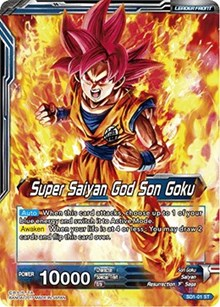
\includegraphics[width=110px]{SD1-01ST.jpg}
%    \caption{Super Saiyan God Son Goku}
%    \label{Super Saiyan God Son Goku}
%  \end{center}
%\end{figure}

%$(\alpha + \beta)^2 = \alpha^2 + \beta^2 + 2\alpha\beta$

\end{document}
